\documentclass[sigconf,nonacm]{acmart}
\usepackage{booktabs}

\settopmatter{printacmref=false, printccs=false, printfolios=true}
\renewcommand\footnotetextcopyrightpermission[1]{}
\pagestyle{plain}

\begin{document}

\title[Leakage-Aware Event-State Forecasting]{Leakage-Aware Deep Learning for Financial Event-State Forecasting}

\author{Jose Ignacio Valdivia Aguero}
\affiliation{%
  \institution{University of Luxembourg}
  \country{Luxembourg}
}

\begin{abstract}
This project studies aligned company-news event states for multi-horizon excess-return forecasting beyond strong market baselines. I built a local, reproducible artifact pipeline for the top-50 liquid U.S. equities, with same-day-as-close news alignment, no-news states, purged expanding folds, an untouched lockbox, fold-local preprocessing, saved predictions, and tuning ledgers. The primary XGBoost configuration completed 800 development trials and is the strongest lockbox error model: weighted error improved by $-5.34\times10^{-4}$ versus the prior XGBoost baseline with a 62.2\% both-metric improvement rate. TSMixer is the strongest lockbox portfolio-ranking model, reaching 15.05\% over the 137-day lockbox simulation. The Mixed model improved validation by $-2.97\times10^{-4}$ versus XGBoost, but worsened lockbox error by $+9.20\times10^{-5}$. The result is objective-specific: XGBoost wins calibrated error forecasting, while TSMixer wins ranking-driven portfolio simulation.
\end{abstract}

\maketitle

\section{Introduction}
Financial news may contain useful short-lived information, but return prediction is low signal-to-noise and highly vulnerable to leakage, multiple testing, and post-hoc narratives. The project therefore frames the task as end-of-day forecasting of forward excess returns for horizons $\{1,5,10,20,60\}$ days. The contribution is a reproducible deep-learning-ready benchmark: top-50 equities, Alpha Vantage news, Twelve Data OHLCV, explicit no-news rows, purged walk-forward development folds, a final lockbox, and artifact-backed model comparisons. The implemented roster spans linear and tree market baselines, FinBERT feature sidecars, TSMixer sequence models, XGBoost tuning, and horizon-level XGBoost/TSMixer mixing. AUC is intentionally not reported: the target is continuous excess return, so RMSE/MAE, zero-baseline $R^2$, rank IC, bootstrap support, and lockbox deltas are the relevant metrics.

\begin{figure*}[t]
  \centering
  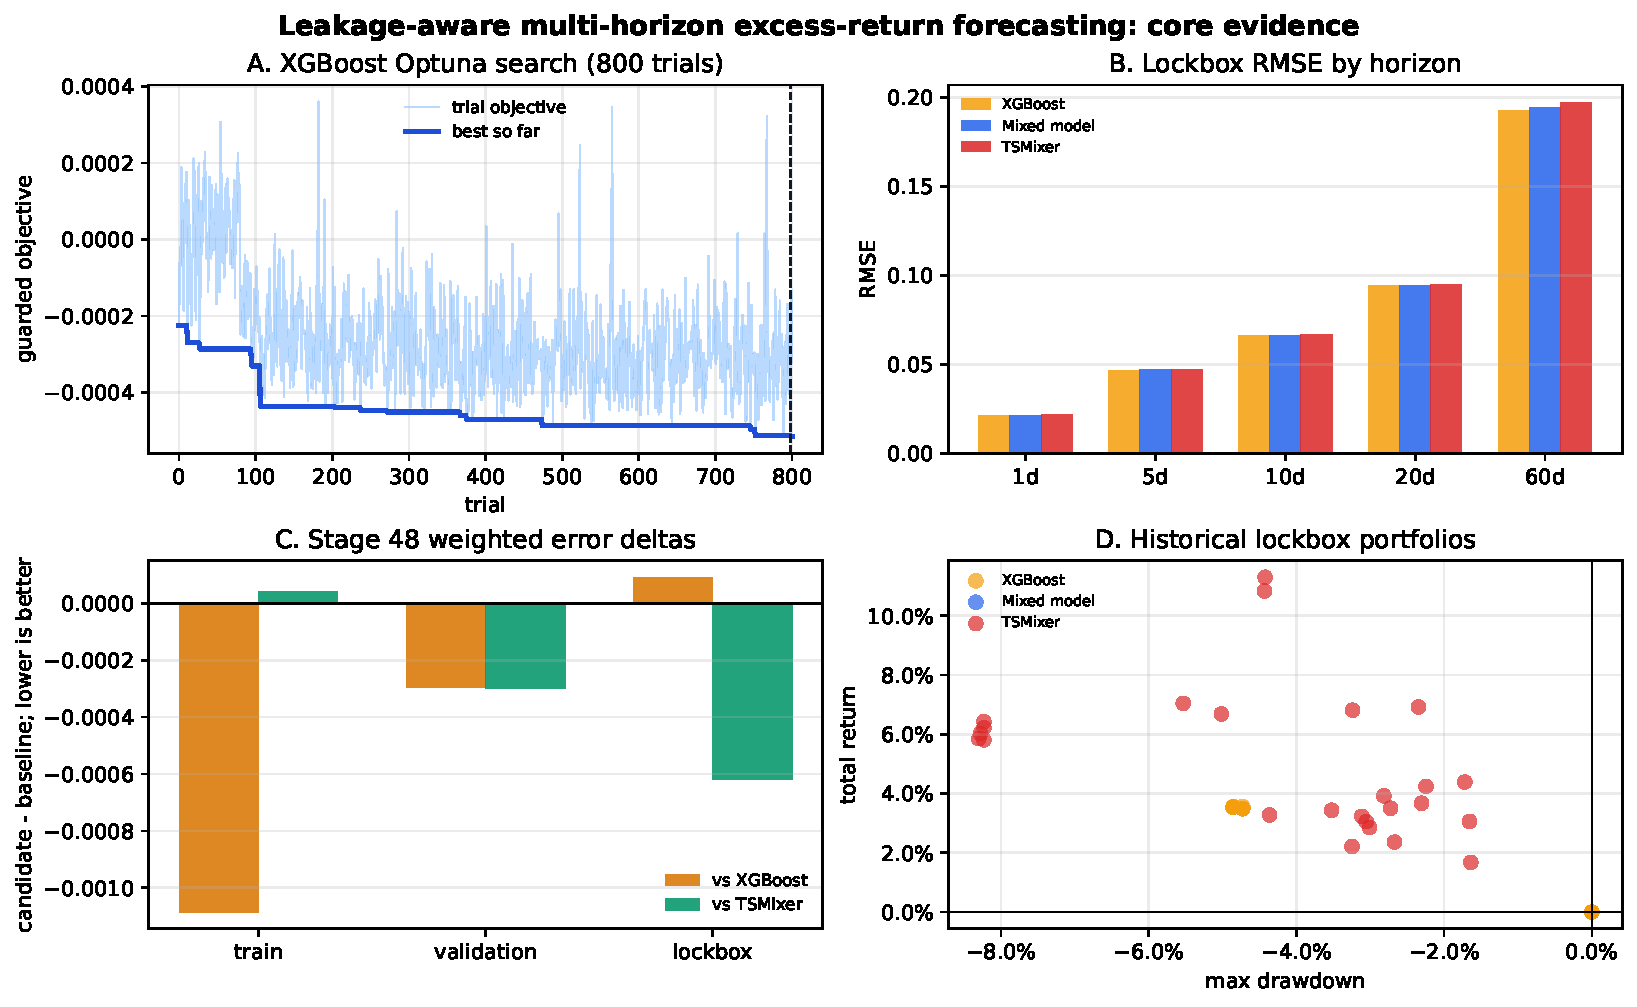
\includegraphics[width=0.98\textwidth]{report_artifacts/main_results_panel.pdf}
  \caption{Core evidence. A: XGBoost tuning used train/validation-only selection. B: lockbox RMSE by horizon. C: Mixed model validation gains did not transfer to lockbox. D: the lockbox portfolio simulation summarizes realized forecast rankings over the 137-day evaluation window.}
  \Description{Four-panel figure showing tuning objective, RMSE bars, weighted error deltas, and portfolio return versus drawdown.}
  \label{fig:main}
\end{figure*}

\section{Related Work}
The design follows market-efficiency and asset-pricing principles from Fama, Fama-French, and Campbell-Lo-MacKinlay \cite{Fama1970,FamaFrench1993,Campbell1997}: small apparent edges require strict out-of-sample controls. Textual-finance work shows why news can matter but also why representation matters \cite{Tetlock2007,LoughranMcDonald2011}. Modern NLP motivates contextual encoders and FinBERT-style finance adaptation \cite{Devlin2019BERT,Araci2019FinBERT}. For tabular market features, gradient boosting remains a strong baseline \cite{ChenGuestrin2016,Ke2017LightGBM}. For sequence modeling, the relevant state of the art includes interpretable multi-horizon attention, patch-based transformers, inverted transformers, and foundation time-series models \cite{Lim2021TFT,Nie2023PatchTST,Liu2024iTransformer,Ansari2024Chronos}. Evaluation follows forecasting-metric and time-series validation guidance \cite{HyndmanKoehler2006,Bergmeir2018}; multiple-testing control follows Harvey et al. \cite{Harvey2016}. ROC-AUC is cited only to justify exclusion for this regression target \cite{Fawcett2006}.

\section{Experiments}
\textbf{Data and splits.} The benchmark uses 50 liquid equities, five horizons, forward leave-one-out excess-return labels, and explicit event-state rows for no-news dates. The enhanced Alpha Vantage rebuild aligned 166,711 news rows while preserving provider-truncation limitations. The split protocol defines nine expanding walk-forward development folds plus a held-out lockbox from 2025-09-30 to 2026-02-13; lockbox rows are never used for tuning.

\begin{table}[t]
\centering
\scriptsize
\caption{Protocol: Leakage-aware artifact pipeline.}
\begin{tabular}{@{}p{0.12\linewidth}p{0.26\linewidth}p{0.30\linewidth}p{0.18\linewidth}@{}}
\toprule
Stage & Artifact & Key control & Output \\
\midrule
Data & Top-50 + OHLCV + news & no raw overwrite & row universe \\
Features & market + event states & no-news rows preserved & sidecars \\
Splits & expanding folds + lockbox & purge/embargo & split manifest \\
Training & fold-local preprocessing & no lockbox tuning & saved preds \\
Evaluation & RMSE/MAE + rank IC & bootstrap + lockbox & reports \\
\bottomrule
\end{tabular}
\vspace{0.25em}

\parbox{0.95\linewidth}{\scriptsize Horizons: 1d, 5d, 10d, 20d, 60d. Lockbox ends 2026-02-13; all result roots keep manifests and prediction packets.}
\label{tab:protocol}
\end{table}

\textbf{Models and training.} XGBoost is the primary event-market candidate, selected from the full 800-trial Optuna search. Its short-horizon portfolio rankings are flat for the 1d and 5d simulations, which identifies a concrete signal-construction issue for the next portfolio simulation. The TSMixer branch remains a frozen sequence-model comparator, and the Mixed model is a lightweight frozen-base horizon mixer over XGBoost and TSMixer predictions; no TSMixer weights were retrained.

\textbf{Results.} Figure~\ref{fig:main} shows the key pattern. XGBoost is the strongest active model on lockbox error metrics: per-horizon RMSE is 0.0214, 0.0468, 0.0661, 0.0943, and 0.1929 for 1d, 5d, 10d, 20d, and 60d respectively (Appendix Table~\ref{tab:lockbox_horizon_results}). TSMixer is the strongest lockbox ranking model in the portfolio simulation: every best-by-horizon portfolio row is TSMixer, including 15.05\% at 1d and 12.43\% at 60d (Appendix Table~\ref{tab:portfolio_horizon_results}). The Mixed model improved validation fit but did not beat XGBoost on lockbox error. Thus, error forecasting and cross-sectional ranking produce different winners.

\section{Discussion}
The strongest lesson is that financial deep learning must be evaluated as a full forecasting system, not as an isolated model leaderboard. XGBoost is the best calibrated error forecaster because it improves the prior XGBoost lockbox weighted error and clears more than half of RMSE/MAE comparisons. TSMixer is the best ranking forecaster because its sequence predictions translate most strongly into lockbox portfolio simulations. The Mixed model adds scientific value by showing that strong validation performance does not automatically translate to lockbox performance. Next steps are to try a deeper reinforcement learning model with capacity to rank predictions from most probable to least probable, expand data collection beyond the 25-call/day API bottleneck, and add transaction costs for richer portfolio evaluation. The project therefore produces a strong excess-return forecasting benchmark, an objective-specific model conclusion, and a concrete roadmap for improving the next model family.

\clearpage

\bibliographystyle{ACM-Reference-Format}
\bibliography{FinalReport}

\clearpage
\onecolumn

\appendix

\section{Artifact Roots and Replication Commands}
\begingroup\scriptsize\sloppy
Repository: \url{https://github.com/ValdiviaEng/financial-event-state-forecasting.git}. Primary evidence roots are XGBoost \url{data/v1p0_full_results/v1p0__phase1_top50_updated_av__stage43__xgboost_tuning__20260528T100000Z__src_6dff1bd__run_40f1c9a0/}, the Mixed model \url{data/v1p0_full_results/v1p0__phase1_top50_updated_av__stage48__frozen_tsmixer_horizon_mixer__20260529T093301Z__src_6dff1bd__run_fc4c1756/}, and the lockbox portfolio simulation \url{data/v1p0_full_results/v1p0__phase1_top50_updated_av__stage47__lockbox_portfolio_simulation__20260529T095157Z__src_6dff1bd__run_8317929b/}. Validation command: \texttt{source \string~/venvs/ai/bin/activate \&\& python -m pytest tests}.
\endgroup

\section{Exact Lockbox Results}
\begin{table}[H]
\centering
\small
\caption{Lockbox metrics by model and horizon. Lower RMSE/MAE is better; $R^2$ is against the zero-return baseline.}
\begin{tabular}{@{}llrrr@{}}
\toprule
Model & Horizon & RMSE & MAE & $R^2$ \\
\midrule
XGBoost & 1d & 0.0214 & 0.0146 & 0.0000 \\
TSMixer & 1d & 0.0221 & 0.0154 & -0.0640 \\
Mixed model & 1d & 0.0214 & 0.0146 & -0.0000 \\
XGBoost & 5d & 0.0468 & 0.0335 & 0.0000 \\
TSMixer & 5d & 0.0469 & 0.0337 & -0.0085 \\
Mixed model & 5d & 0.0469 & 0.0336 & -0.0058 \\
XGBoost & 10d & 0.0661 & 0.0488 & 0.0000 \\
TSMixer & 10d & 0.0670 & 0.0494 & -0.0262 \\
Mixed model & 10d & 0.0665 & 0.0490 & -0.0101 \\
XGBoost & 20d & 0.0943 & 0.0696 & -0.0014 \\
TSMixer & 20d & 0.0949 & 0.0701 & -0.0148 \\
Mixed model & 20d & 0.0944 & 0.0696 & -0.0031 \\
XGBoost & 60d & 0.1929 & 0.1396 & 0.0072 \\
TSMixer & 60d & 0.1972 & 0.1398 & -0.0374 \\
Mixed model & 60d & 0.1942 & 0.1384 & -0.0063 \\
\bottomrule
\end{tabular}
\label{tab:lockbox_horizon_results}
\end{table}

\begin{table}[H]
\centering
\small
\caption{Best portfolio row by horizon over the 137-day lockbox interval. The rows summarize realized forecast-ranking simulations under the stated frictionless assumptions.}
\begin{tabular}{@{}llrrr@{}}
\toprule
Horizon & Model / policy & Return & Final equity & Trades \\
\midrule
1d & TSMixer / one\_d\_bot10 & 15.05\% & \$115,045 & 1161 \\
5d & TSMixer / one\_d\_bot10 & 5.24\% & \$105,240 & 1831 \\
10d & TSMixer / none & 9.48\% & \$109,482 & 1780 \\
20d & TSMixer / none & 7.54\% & \$107,536 & 1680 \\
60d & TSMixer / botk\_3\_of\_5 & 12.43\% & \$112,434 & 1319 \\
\bottomrule
\end{tabular}
\label{tab:portfolio_horizon_results}
\end{table}

\section{Supplementary Visualizations}

\begin{figure}[H]
  \centering
  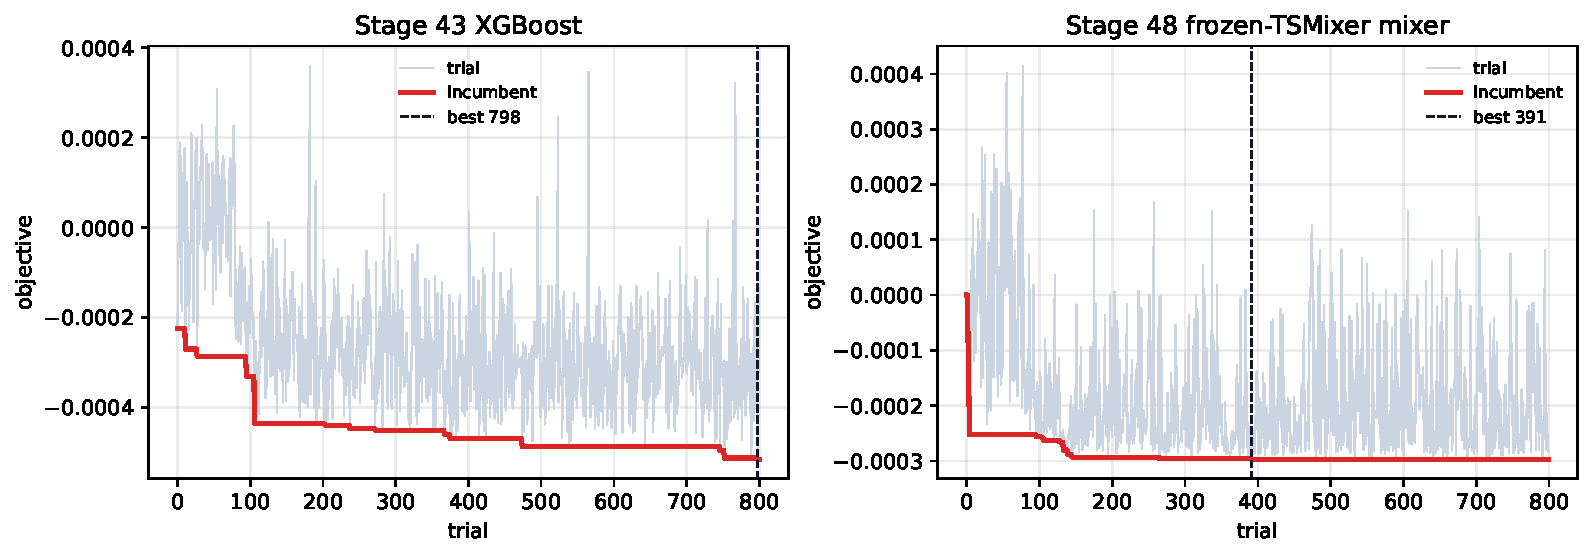
\includegraphics[width=\linewidth]{report_artifacts/tuning_curves.pdf}
\caption{Optuna incumbent curves for XGBoost and the Mixed model.}
  \Description{Two line plots of trial objective and best-so-far objective.}
\end{figure}

\begin{figure}[H]
  \centering
  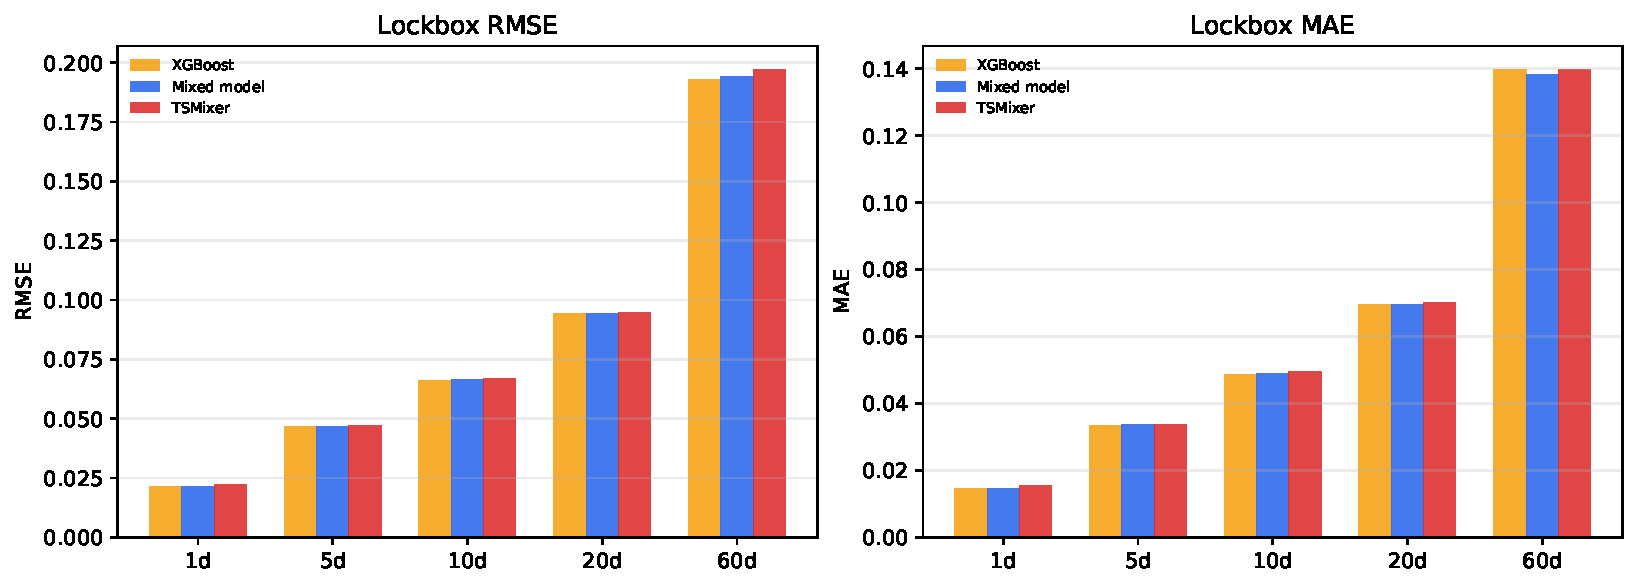
\includegraphics[width=\linewidth]{report_artifacts/lockbox_rmse_mae.pdf}
\caption{Lockbox RMSE and MAE by horizon for XGBoost, TSMixer, and the Mixed model.}
  \Description{Grouped bar charts of RMSE and MAE over five forecast horizons.}
\end{figure}

\begin{figure}[H]
  \centering
  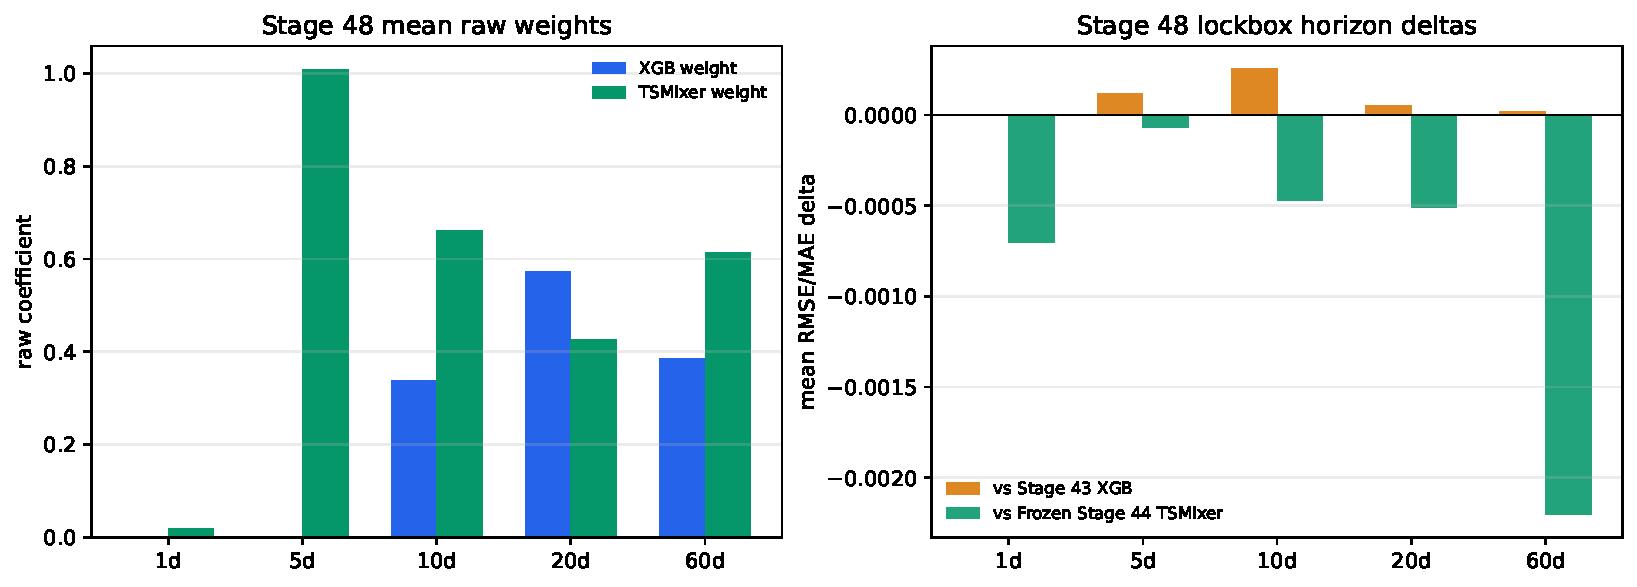
\includegraphics[width=\linewidth]{report_artifacts/mixer_weights_deltas.pdf}
\caption{Horizon-specific raw mixer weights and lockbox horizon deltas.}
\Description{Bar charts of XGBoost and TSMixer weights and candidate-minus-baseline deltas.}
\end{figure}

\begin{figure}[H]
  \centering
  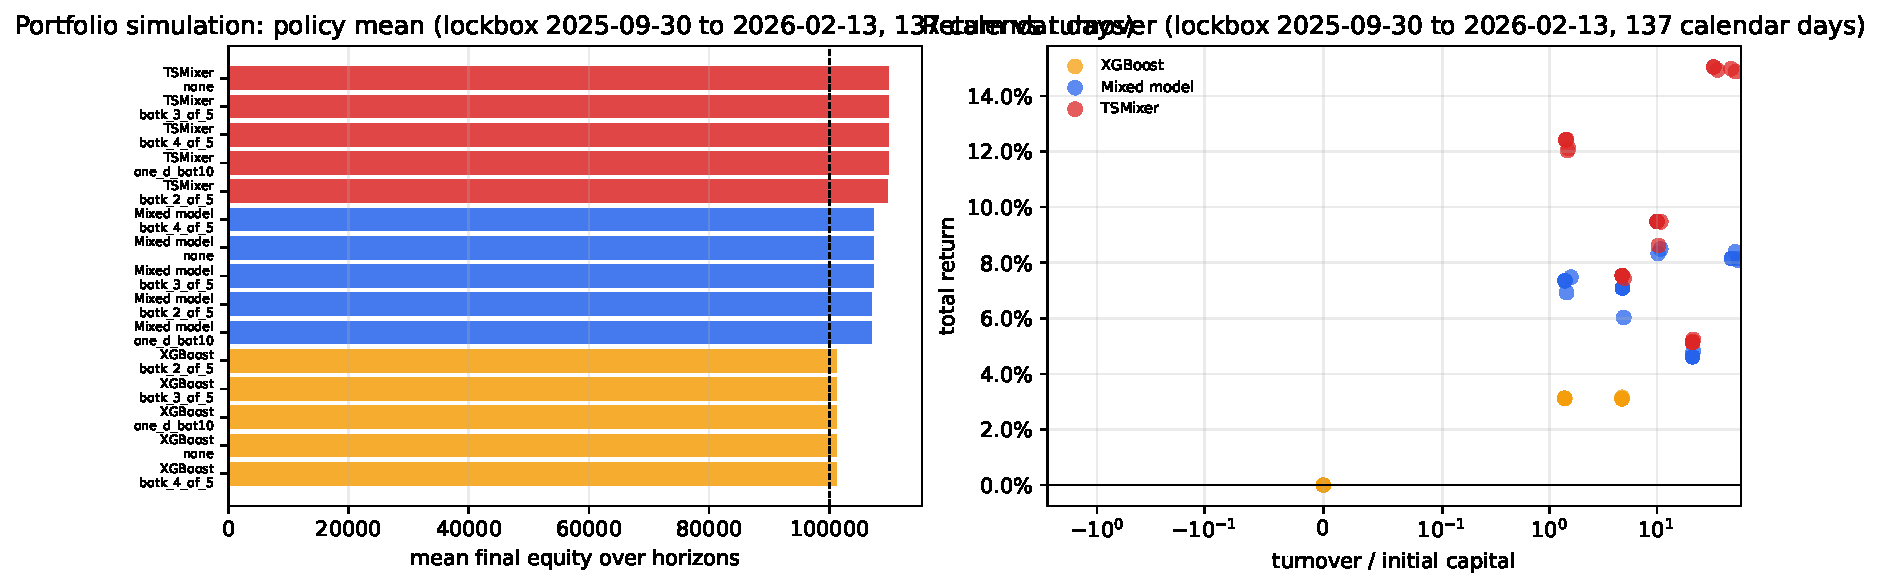
\includegraphics[width=\linewidth]{report_artifacts/portfolio_simulations.pdf}
\caption{Portfolio simulations over the 2025-09-30 to 2026-02-13 lockbox interval (137 calendar days): final equity by policy and return versus turnover.}
\Description{Horizontal bar chart and scatter plot for portfolio simulations.}
\end{figure}

\begin{figure}[H]
  \centering
  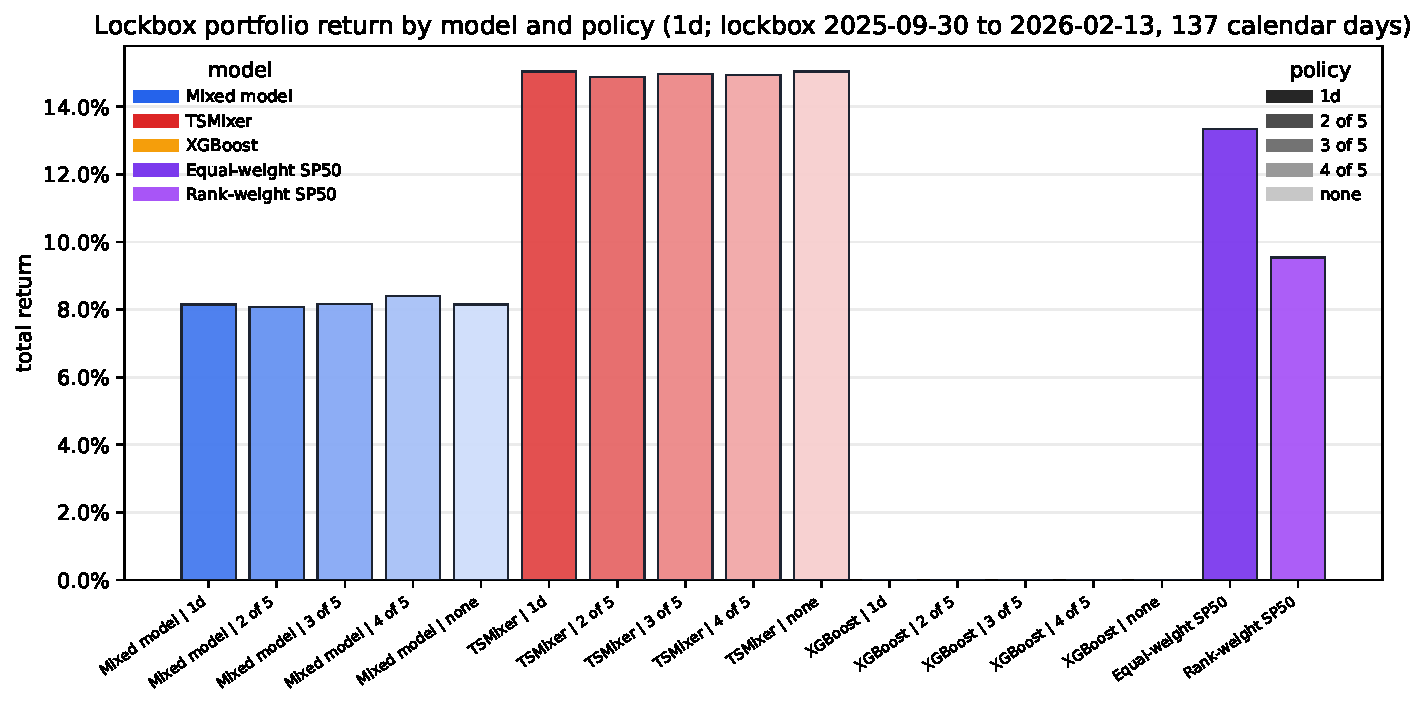
\includegraphics[width=0.48\linewidth]{report_artifacts/portfolio_returns_by_policy_model_1d.pdf}\hfill
  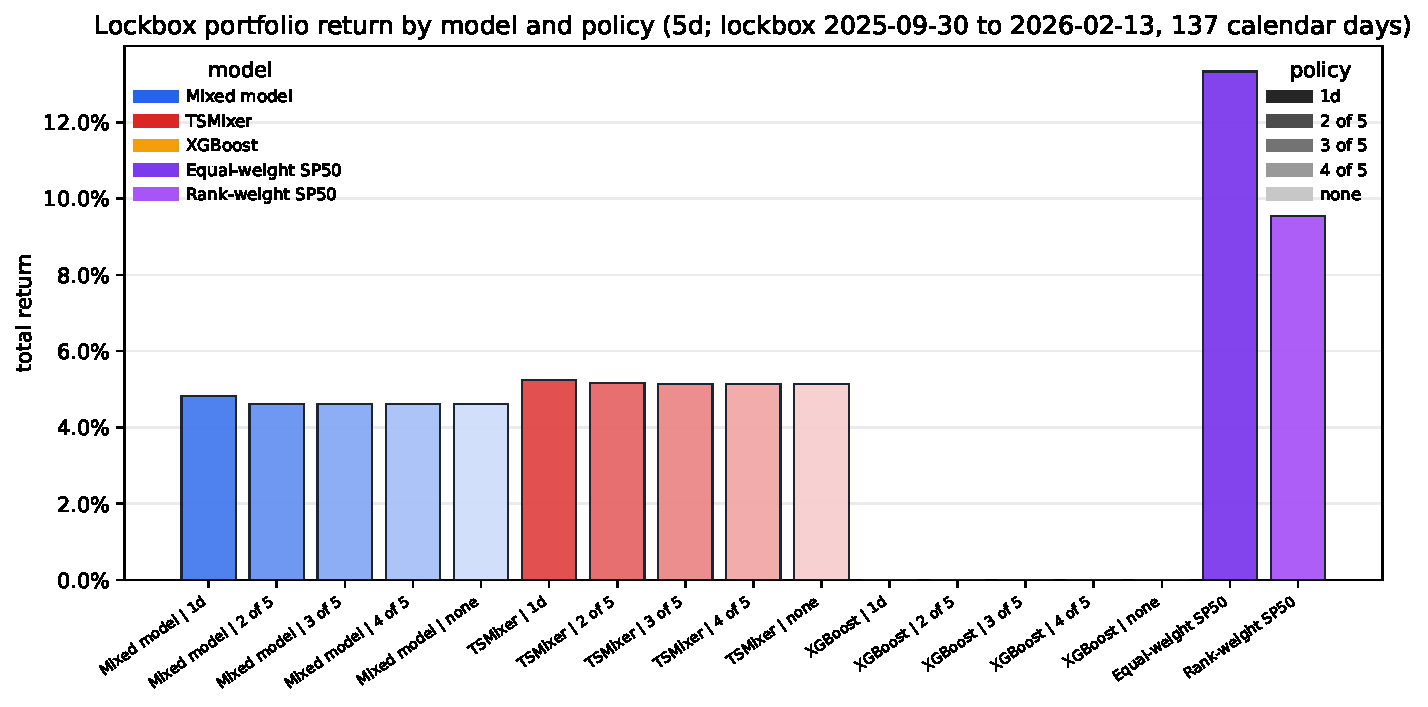
\includegraphics[width=0.48\linewidth]{report_artifacts/portfolio_returns_by_policy_model_5d.pdf}
  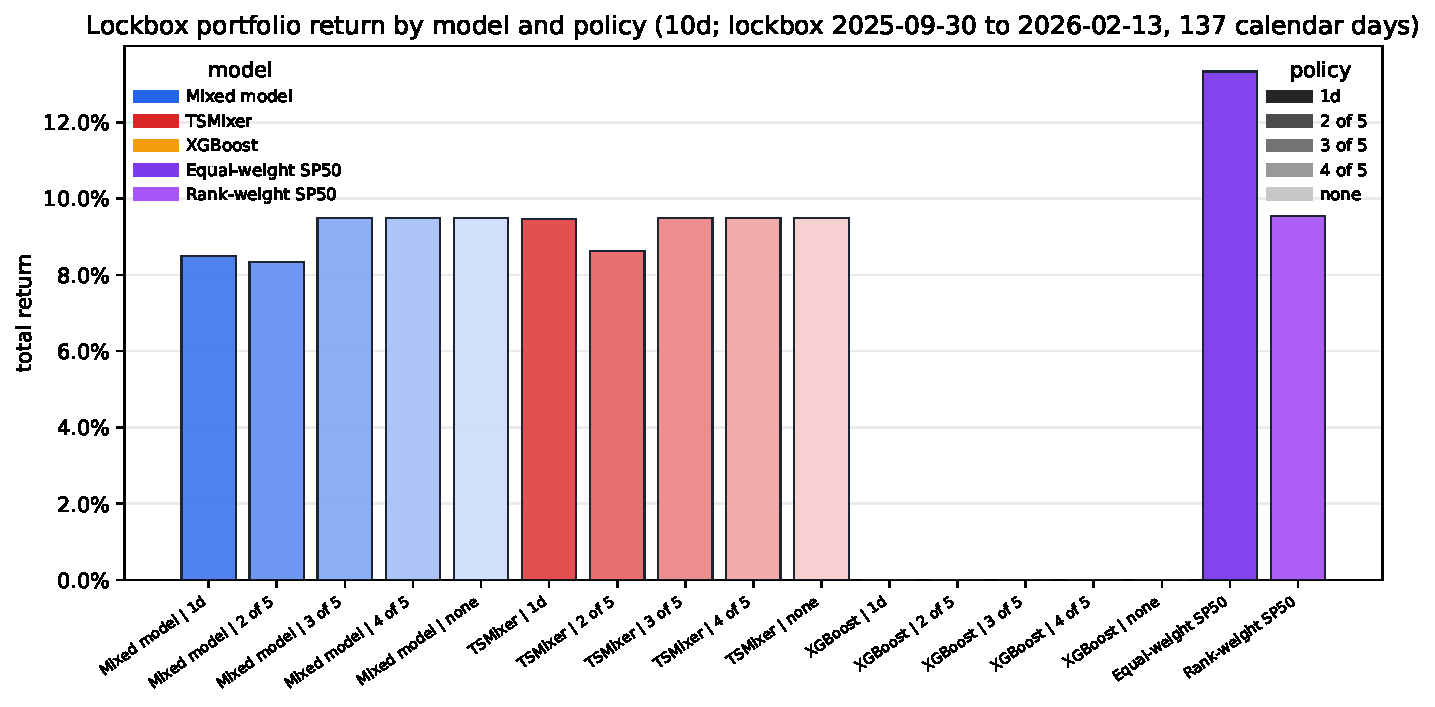
\includegraphics[width=0.48\linewidth]{report_artifacts/portfolio_returns_by_policy_model_10d.pdf}\hfill
  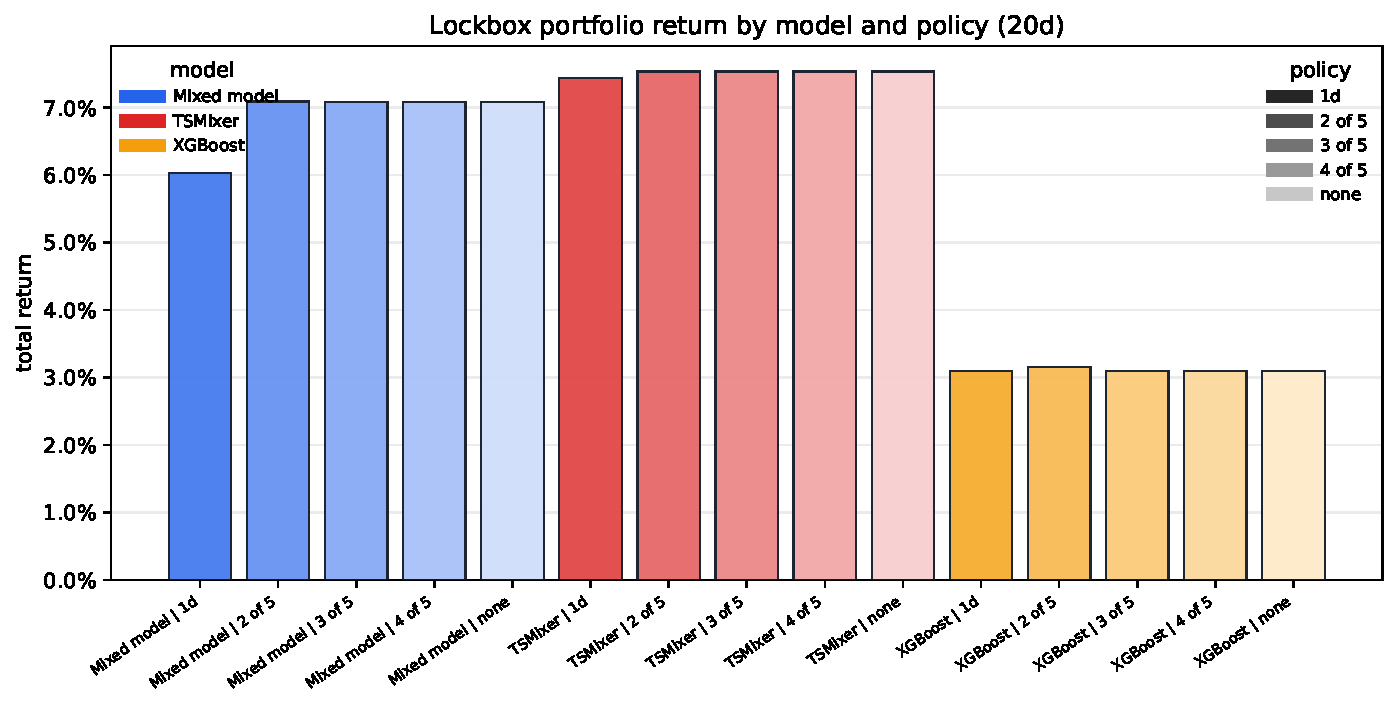
\includegraphics[width=0.48\linewidth]{report_artifacts/portfolio_returns_by_policy_model_20d.pdf}
  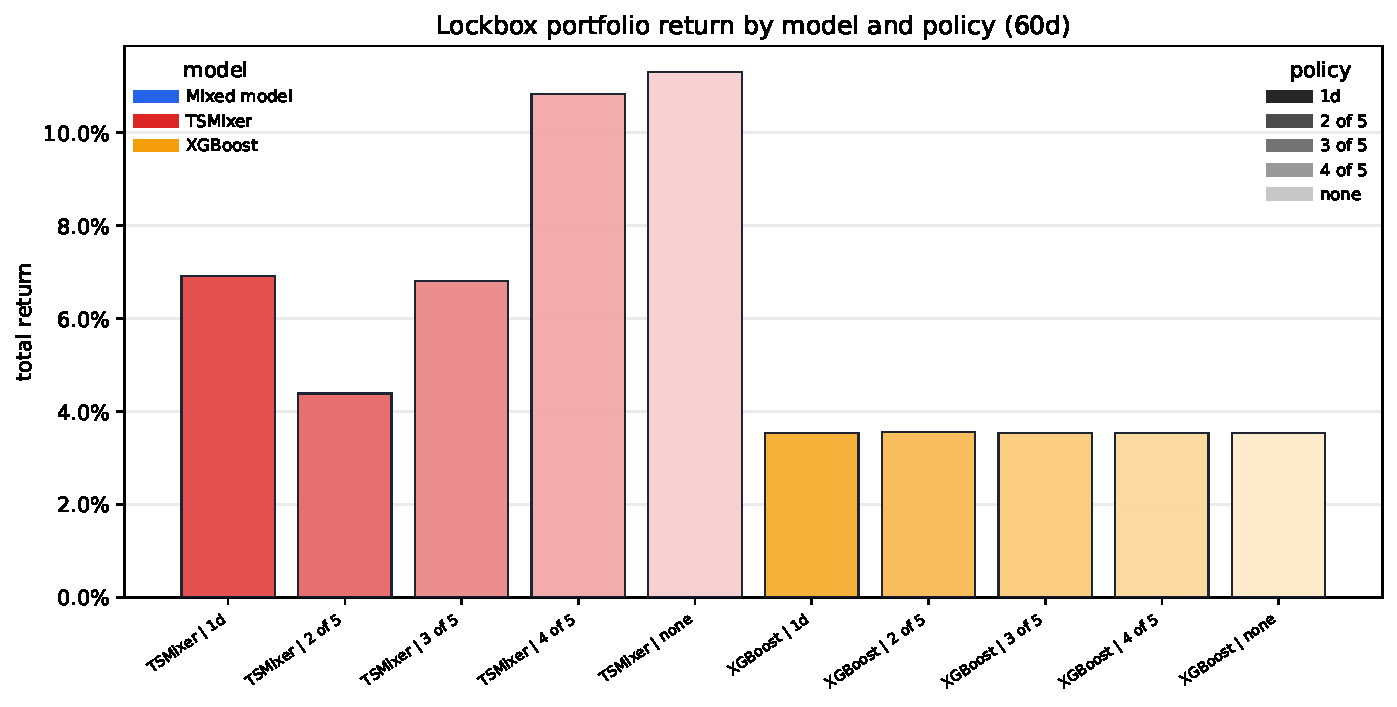
\includegraphics[width=0.48\linewidth]{report_artifacts/portfolio_returns_by_policy_model_60d.pdf}
\caption{Portfolio return bars by horizon, model, sell policy, and SP50 benchmark proxy over the 137-day lockbox interval.}
  \Description{Five bar charts of portfolio returns by model and policy for each horizon with SP50 proxy bars.}
\end{figure}

\begin{figure}[H]
  \centering
  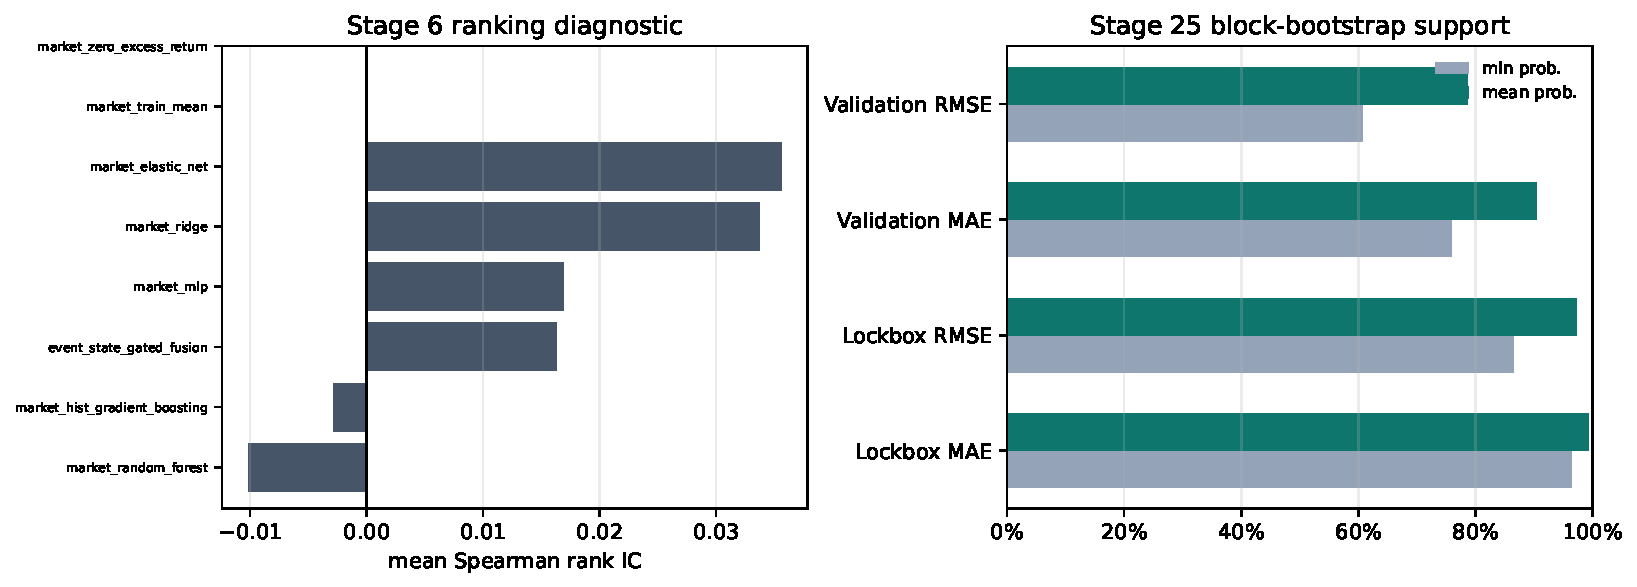
\includegraphics[width=\linewidth]{report_artifacts/ranking_uncertainty.pdf}
  \caption{Ranking signal quality and block-bootstrap support.}
  \Description{Rank IC bars and bootstrap improvement probability bars.}
\end{figure}

\end{document}
